\documentclass[a4paper,11pt]{article}
%Premeable
	%Chinese
	\usepackage[UTF8,fontset=fandol]{ctex}
	\usepackage{xeCJK}
	\usepackage[datesep=/]{datetime2}
	\DeclareTextFontCommand{\textbf}{\sffamily}
%Presenting
	\usepackage[table]{xcolor}
	\usepackage{graphicx}
	\usepackage[font={sf}]{caption}
	\usepackage[above]{placeins}
	\usepackage{float,wrapfig}
	\usepackage{tabularx,array,booktabs,multirow,bigstrut}
	\newcolumntype{C}[1]{>{\hsize=#1\hsize%
		\centering\arraybackslash}X}
	\newcommand{\minitab}[2][l]{%
		\begin{tabular}{#1}#2\end{tabular}}
%MathSetting
	\let\latexointop\ointop
	\usepackage{amsmath,bm,amssymb,esint,extarrows}
	\usepackage{upgreek,textcomp,mathrsfs}
	\usepackage[only,sslash]{stmaryrd}
	\usepackage{nicefrac,eqnarray}
%	\usepackage{amsthm}
	\usepackage{mathtools,physics,siunitx}
	\usepackage{stackengine,titling,varwidth}
	\usepackage{tikz}
	\usepackage{resizegather,empheq}
	\usetagform{default}
	\usepackage{calligra,fourier-orns}
	% Keep \oint unchanged by esint
	\let\ointop\undefined
	\let\ointop\latexointop
	% Define a scriptr 
	\DeclareMathAlphabet{\mathcalligra}{T1}{calligra}{m}{n}
	\DeclareFontShape{T1}{calligra}{m}{n}{<->s*[2.2]callig15}{}
	\newcommand{\scriptr}{\mathcalligra{r}\,}
	\newcommand{\rvector}{\pmb{\mathcalligra{r}}\,}
	% Useful shorthand
	\DeclarePairedDelimiter\ave{\langle}{\rangle}
	\newcommand\inlineeqno{\stepcounter{equation}\ (\theequation)}
	\newcommand{\sinc}{\operatorname{sinc}}
	\newcommand{\mbb}[1]{\mathbb{#1}}
	\newcommand{\mrm}[1]{\mathrm{#1}}
	\newcommand{\mcal}[1]{\mathcal{#1}}
	% Scaling and positioning
	\newcommand\scalemath[2]{\scalebox{#1}{\mbox{\ensuremath{\displaystyle #2}}}}
	\newcommand\raisemath[2]{\raisebox{#1\depth}{${#2}$}}
	\empheqset{box=\bbox}
	% Presenting
	\newcommand*\bbox[1]{\fbox{\hspace{1em}\addstackgap[5pt]{#1}\hspace{1em}}}
	\sisetup{%
		redefine-symbols=false,%
		separate-uncertainty=true,%
		range-phrase=\,\textasciitilde\,,%
		arc-separator = \,}
	\allowdisplaybreaks[2]
%ParagraphSetting
	\setlength{\parskip}{.3\baselineskip}
	\usepackage[defaultlines=2,all]{nowidow}
	\postdisplaypenalty=50
%PageSetting
	\usepackage[colorlinks=true,linkcolor=blue]{hyperref}
	\usepackage[vmargin={4cm,5cm},hmargin=3cm,%
		footnotesep=\baselineskip]{geometry}
	\usepackage[bottom]{footmisc}
	\usepackage{changepage}
	% Autoref names
	\renewcommand{\tableautorefname}{\tablename}
	\renewcommand{\figureautorefname}{\figurename}
	% List settings
	\usepackage{enumitem}
	\setlist{itemsep=0pt,topsep=0pt,labelindent=\parindent,leftmargin=0pt,itemindent=*}
	% Some redefined lengths
	\setlength{\headsep}{2.2cm}
	\setlength{\droptitle}{-2.2cm}
	\setlength{\footnotesep}{3\parskip}
	% Header
	\usepackage{fancyhdr,lastpage}
	\pagestyle{fancy}
	\fancyhf{}
	\cfoot{--\ \thepage\,/\,\pageref{LastPage} \ --}
	\renewcommand{\headrulewidth}{0.1pt}
	\renewcommand{\headrule}{
		\vbox to 2pt{
		\hbox to \headwidth{\dotfill}\vss}}
	% Separator
	\newcommand{\newparagraph}{\pagebreak[3]\noindent%
		\hfil
		~\raisebox{-4pt}[10pt][10pt]{\decofourright~~~~~~~~\decofourleft}~ %
		\par
	}
%TitleSettings
	\pretitle{\begin{center}}
	\posttitle{\par\end{center}\vspace{-6mm}}
	\predate{}
	\postdate{\vspace{-4mm}}
%Header
	\lhead{%
		
\includegraphics[height=3.2em]{PKUPhy.png}
		\vspace{-3ex}
		}
	\rhead{%
		\itshape\small
		\begin{tabular}{rr}
			\multicolumn{2}{r}{赵启渊} \\[.3em]
			学号:   & 2000011153 \\[.2em]
		\end{tabular}\hspace{-1em}
		}
%Title
	\title{\textit{\large 实验八}\\[2mm]
		\textbf{\LARGE 测量金属的杨氏模量}}
	\author{\textit{赵启渊} 2000011153}
	\date{}
%Miscellaneous
	\newcommand{\tabindent}{\hspace{2em}}
%FourierTransform
	\newcommand{\ftransform}{\xlongrightarrow{\ \mathscr F\ }}
	\newcommand{\iftransform}{\xlongrightarrow{\ \mathscr F^{-1}\ }}
	\usepackage{gensymb}

\begin{document}
	\vspace*{1cm}
	
	\vspace*{1cm}
	
	\begin{center}
		\Huge{\textbf{基础物理实验报告}}
		
		\Large{测量金属的杨氏模量}
	\end{center}
	
	\vspace*{2cm}
	
	\begin{table}[h]
		\centering	
		\begin{Large}
			\begin{tabular}{p{3cm} p{7cm}<{\centering}}
				姓\qquad 名: & 赵启渊 \\
				\hline
				学\qquad 院: & 工学院 \\
				\hline
				学\qquad 号: & 2000011153 \\
				\hline
				分\qquad 组: & 第1组7号 \\
				\hline
				日\qquad 期: & 2022年4月27日 \\
				\hline
				指导教师: & 刘春玲\ 夏颖\\
				\hline
			\end{tabular}
		\end{Large}
	\end{table}
	
\maketitle
\thispagestyle{fancy}
\section{数据及处理}
\subsection{CCD成像系统测定杨氏模量}
\subsubsection{相关数据的测量}
在调试好实验装置之后,称量每个砝码的重量,并测量金属丝受外力拉伸后的伸展变化数据,再测量金属丝长L和金属丝直径d。其中,有$ \delta L = (\bar{r}_{i+5} - \bar{r}_{i})  $ 
\begin{table}[H]
	\centering\caption{CCD法测量金属丝受外力拉伸后的伸展变化数据表}
	\small
	\begin{tabularx}{.85\linewidth}{C{1} *5{C{1}}}
		\toprule
		\textbf{i} &
		$ m_{i}/g $ &
		$ r_{i}/cm $ &
		$ r_{i}^{\prime}/cm $ &
		$ \bar{r}/cm $ &
		$ \delta L  /cm $\\
		\midrule
		0     & 0  & 0.235 & 0.235 &  0.235 &     \\
		1     & 199.96  & 0.235 & 0.235 &  0.235 &     \\
		2     & 199.53  & 0.245 & 0.245 &  0.245 &     \\
		3     & 199.76  & 0.255 & 0.255 &  0.255 &     \\
		4     & 200.41  & 0.265 & 0.265 &  0.265 &     \\
		5     & 199.93  & 0.280 & 0.275 &  0.278 & 0.043    \\
		6     & 200.06  & 0.290 & 0.290 &  0.290 & 0.055    \\
		7     & 199.91  & 0.300 & 0.300 &  0.300 & 0.055    \\
		8     & 199.97  & 0.315 & 0.310 &  0.312 & 0.057    \\
		9     & 199.96  & 0.325 & 0.325 &  0.325 & 0.060    \\
		\bottomrule
	\end{tabularx}
	\vspace{3ex}
\end{table}\noindent%

金属丝长 L = 100.00 - 21.10 = 78.90 cm \\
\\
\\
\\
\\
\\


	\begin{table*}[htbp]%调节图片位置,h:浮动;t:顶部;b:底部;p:当前位置
	\centering
	\caption{测量金属丝直径数据表}
	\label{tab:1}  
	\begin{tabular}{cccc ccccccc}
		\hline\hline\noalign{\smallskip}	
		i  & 1 & 2 & 3 & 4 & 5 & 6 & 7 & 8 & 9 & 10   \\
		\noalign{\smallskip}\hline\noalign{\smallskip}
		$ d^{\prime}/cm $ & 0.0321 & 0.0321 & 0.0322  & 0.0323 & 0.0321 & 0.0325 & 0.0324 & 0.0323 & 0.0322 & 0.0324     \\
		\noalign{\smallskip}\hline
		
	\end{tabular}
\end{table*}

测量得到 $d_0$ = 0.0000 cm,
上面有 $ d^{\prime} = d - d_0 $\\
计算得$$ \bar{d^{\prime}} = 0.0323 cm $$

\subsubsection{记录一次测量数据的不确定度}
$$ e_{L} = 0.1 cm $$

\subsubsection{用逐差法和最小二乘法分别处理数据}
使用最小二乘法处理$ \bar{r} - m $可以得到
\begin{figure}[H]
	\centering
	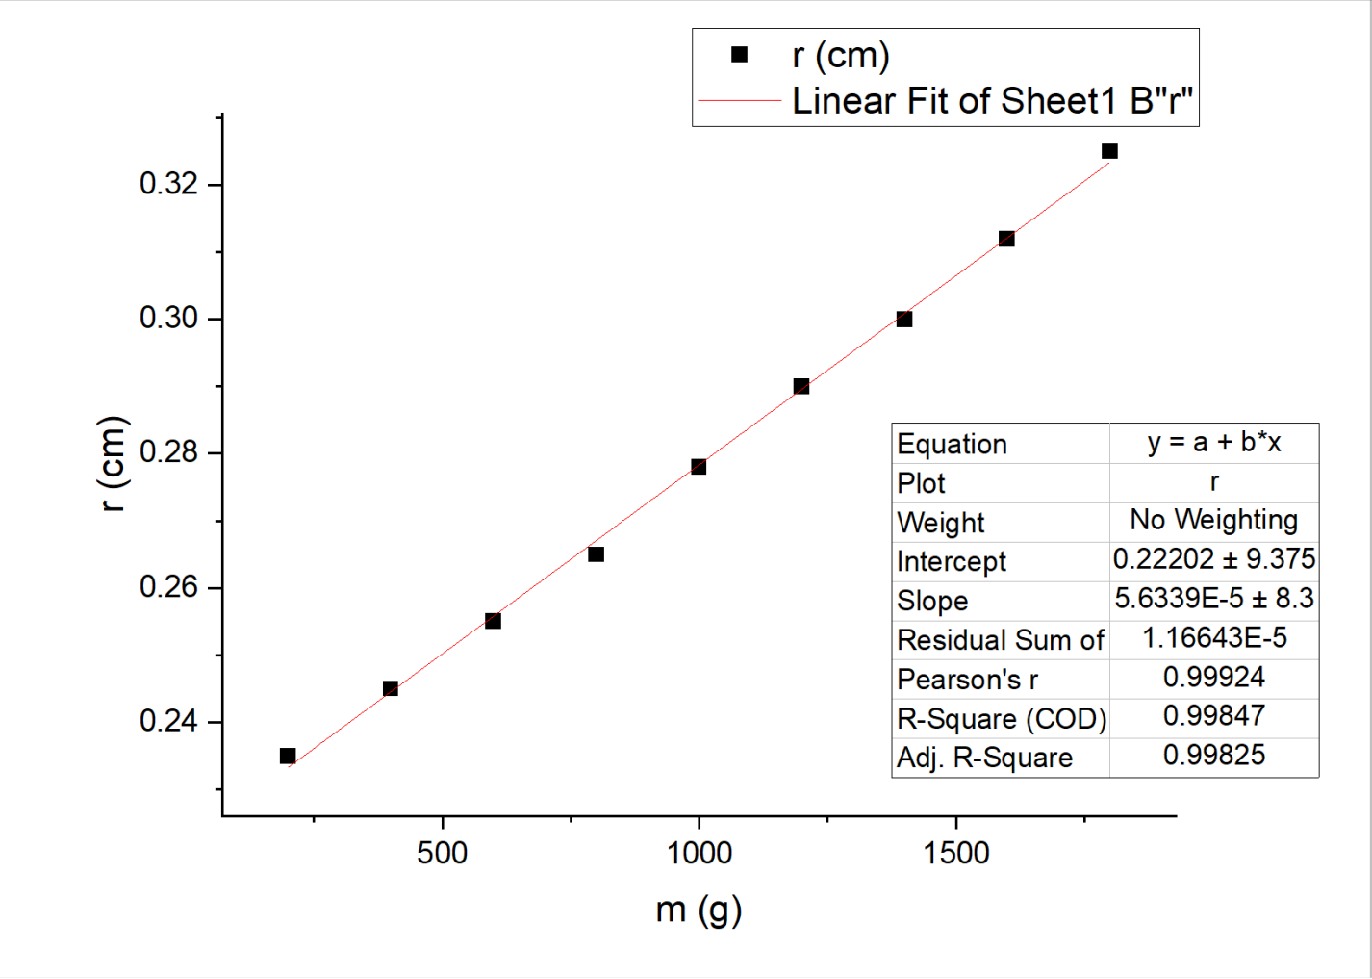
\includegraphics[width=.8\linewidth]{图片1.png}
	\caption{ 测得$ \bar{r} - m $关系图}
\end{figure}\noindent%
其中可以得到$$ a = 5.63 * 10^{-5} $$
$$ b = 0.222 $$
$$ r = 0.99924 $$

使用逐差法处理数据$$  \bar{\delta L} = \dfrac{(\bar{r_6} - \bar{r_1})+(\bar{r_7} - \bar{r_2})+(\bar{r_8} - \bar{r_3})+(\bar{r_9} - \bar{r_4})}{4} $$
$$ = \dfrac{0.055 + 0.055 + 0.057 + 0.060}{4} $$
$$ = 0.057 cm $$
还有$$  \bar{\delta m} = \dfrac{(\bar{m_6} - \bar{m_1})+(\bar{m_7} - \bar{m_2})+(\bar{m_8} - \bar{m_3})+(\bar{m_9} - \bar{m_4})}{4} $$
$$ = \dfrac{999.69 + 1000.07 + 1000.28 + 999.83}{4} $$
$$ = 999.97 g $$
\subsubsection{计算杨氏模量及其不确定度}
在计算时发现,第一组的数据偏离过大,当舍去第一组数据时,计算得到
$$ \bar{\delta L} = 0.057 cm $$
这里$g = 9.8012 N/kg$
$$ \bar{F} = \bar{\delta m} * g  = 9.8009 N  $$
其中有$$ \delta m = m_{i+5} - m_{i} $$
有杨氏模量的计算公式有
$$ E = \dfrac{F * L}{S * \delta L } $$
$$  = \dfrac{F * L * 4}{\pi * d^2 * \delta L } $$
$$ = 1.66 * 10 ^{11} N/m^2 $$

\begin{enumerate}
	\item 计算$\bar{d^{\prime}}$的不确定度:\\
	其中平均值的标准差计算使用$$ \sqrt{\frac{\sum _{j=1}^{n}{\left({N}_{j}-\stackrel{-}{N}\right)}^{2}}{n\left(n-1\right)}} $$
	$$ = \sqrt{\frac{2}{9} * 10^{-8}} cm $$
	$$ = 4.71 * 10^{-5} cm $$
	考虑仪器允差之后的标准差计算使用$$\sqrt{\frac{\sum _{j=}^{n}{\left({N}_{j}-\stackrel{-}{N}\right)}^{2}}{n\left(n-1\right)}+{\left(\frac{e}{\sqrt{3}}\right)}^{2}}$$
	这里$ e_d = 0.004 mm $
	$$\sigma_d = \sqrt{\frac{2}{9} * 10^{-8} + \frac{0.0004^2}{3}} $$
	$$ = 2.36 * 10^{-4} cm $$
	这里可以得到
	$$ \bar{d^{\prime}} \pm \sigma_d = 0.0323 \pm 0.0002 cm $$
	
	\item 计算$\bar{m}$的不确定度:\\
	其中平均值的标准差计算使用$$ \sqrt{\frac{\sum _{j=1}^{n}{\left({N}_{j}-\stackrel{-}{N}\right)}^{2}}{n\left(n-1\right)}} $$
	$$ = \sqrt{\frac{0.20410}{4 *3} } g $$
	$$ = 0.13042 g $$
	考虑仪器允差之后的标准差计算使用$$\sqrt{\frac{\sum _{j=}^{n}{\left({N}_{j}-\stackrel{-}{N}\right)}^{2}}{n\left(n-1\right)}+{\left(\frac{e}{\sqrt{3}}\right)}^{2}}$$
	这里$ e_m = 0.02 g $
	$$\sigma_m = \sqrt{\frac{0.20410}{4 *3} + \frac{0.02^2}{3}} $$
	$$ = 0.13093 g $$
	这里可以得到
	$$ \bar{m} \pm \sigma_m = 999.97 \pm 0.13 g $$
	
	\item 计算$L$的不确定度:\\
	$$ e_{L} = 0.1 cm $$
	
	\item 计算$\bar{\delta L}$的不确定度:\\
	其中平均值的标准差计算使用$$ \sqrt{\frac{\sum _{j=1}^{n}{\left({N}_{j}-\stackrel{-}{N}\right)}^{2}}{n\left(n-1\right)}} $$
	$$ = \sqrt{\frac{17}{4 *3} * 10^{-6} } cm $$
	$$ = 1.19 * 10^{-3} cm $$
	考虑仪器允差之后的标准差计算使用$$\sqrt{\frac{\sum _{j=}^{n}{\left({N}_{j}-\stackrel{-}{N}\right)}^{2}}{n\left(n-1\right)}+{\left(\frac{e}{\sqrt{3}}\right)}^{2}}$$
	这里$ e_\delta L = 0.005 cm $
	$$\sigma_\delta L = \sqrt{\frac{17}{4 *3} * 10^{-6} + \frac{0.05^2}{3}} $$
	$$ = 3.12 * 10^{-3} cm $$
	这里可以得到
	$$ \bar{\delta L} \pm \sigma_\delta L = 0.057 \pm 0.003 cm $$
	根据杨氏模量的公式
	$$ E = \dfrac{m*g * L * 4}{\pi * d^2 * \delta L } $$
	由求导得到相对不确定度公式
	$$ \dfrac{\sigma_{E}}{E} = \sqrt{(\dfrac{\partial \ln(E)}{\partial \bar{d^{\prime}}} * \sigma_{\bar{d^{\prime}}})^{2} + (\dfrac{\partial \ln(E)}{\partial \bar{m}} * \sigma_{\bar{m}})^{2} + (\dfrac{\partial \ln(E)}{\partial L} * \sigma_{L})^{2} + (\dfrac{\partial \ln(E)}{\partial \bar{\delta L}} * \sigma_{\bar{\delta L}})^{2} } $$
	$$ = \sqrt{(\dfrac{2 * \sigma_{\bar{d^{\prime}}}}{\bar{d^{\prime}}})^{2} + (\dfrac{\sigma_{\bar{m}}}{\bar{m}})^{2}  + (\dfrac{\sigma_{L}}{L})^{2}  + (\dfrac{\sigma_{\bar{\delta L}}}{\bar{\delta L}})^{2}  } $$
	总的不确定度
	$$ \sigma_{E} = E * 0.0541  $$
	$$ \sigma_{E} = 0.0898 * 10^{11} Pa $$
	这里可以得到
	$$ E\pm \sigma_E = 1.66 * 10^{11} \pm 0.09 * 10^{11} Pa $$ 
	
	还可以使用最小二乘法分析不确定度:\\
	$$ \delta L = \dfrac{4 * g *L}{\pi * d^2 *E} * m $$
	因此有
	$$ \bar{r} = \dfrac{4 * g *L}{\pi * d^2 *E} * m $$
	所以根据上面的计算
	$$ k = \dfrac{4 * g *L}{\pi * d^2 *E} = a = 5.63 * 10^{-5} cm/g $$
	$$ r = 0.99924 $$
	所以有
	$$ \dfrac{\sigma_k}{k} = \sqrt{\dfrac{\frac{1}{r^2} - 1}{n-2}} $$
	$$ \dfrac{\sigma_k}{k} = 0.014744 $$
	$$ \sigma_k = 0.0830 * 10^{-5} cm/g $$
	从k的值计算E,可以得到
	$$ k = \dfrac{4 * g *L}{\pi * d^2 *E} $$
	$$ E = 1.68 * 10^{11} Pa $$
	又因为
	$$ E = \dfrac{4 * g *L}{\pi * d^2 *k} $$
	$$ \dfrac{\sigma_{E}}{E} = \sqrt{(\dfrac{\partial \ln(E)}{\partial \bar{d^{\prime}}} * \sigma_{\bar{d^{\prime}}})^{2}  + (\dfrac{\partial \ln(E)}{\partial L} * \sigma_{L})^{2} + (\dfrac{\partial \ln(E)}{\partial k} * \sigma_{k})^{2} } $$
	$$ = \sqrt{(\dfrac{2 * \sigma_{\bar{d^{\prime}}}}{\bar{d^{\prime}}})^{2}   + (\dfrac{\sigma_{L}}{L})^{2}  + (\dfrac{\sigma_{k}}{k})^{2}  } $$
	总的不确定度
	$$ \sigma_{E} = E * 0.0193  $$
	$$ \sigma_{E} = 0.0324 * 10^{11} Pa  $$
	这里可以得到
	$$ E\pm \sigma_E = 1.68 * 10^{11} \pm 0.03 * 10^{11} Pa $$ 
	
\end{enumerate}

\subsection{梁的弯曲测定杨氏模量}
\subsubsection{相关数据的测量}
在调试好实验装置之后,称量每个砝码的重量,并测量金属梁中点受外力影响后的挠度变化数据,再测量金属梁长l和金属梁厚h,金属梁宽度a。其中,有$ \delta L = (\bar{r}_{i+3} - \bar{r}_{i})  $ 
\begin{table}[H]
	\centering\caption{梁的弯曲法测量金属梁中点受外力拉伸后的挠度变化数据表}
	\small
	\begin{tabularx}{.85\linewidth}{C{1} *5{C{1}}}
		\toprule
		\textbf{i} &
		$ m_{i}/g $ &
		$ r_{i}/cm $ &
		$ r_{i}^{\prime}/cm $ &
		$ \bar{r}/cm $ &
		$ \lambda  /cm $\\
		\midrule
		0     & 0  & 4.2819 & 4.1234 &  4.2026 &     \\
		1     & 199.96  & 4.1865 & 4.0181 &  4.1023 &     \\
		2     & 199.53  & 4.0889 & 3.9111 &  4.0000 &     \\
		3     & 199.76  & 3.9882 & 3.8143 &  3.9012 & 0.3012    \\
		4     & 200.41  & 3.8846 & 3.7111 &  3.7978 & 0.3045    \\
		5     & 199.93  & 3.7791 & 3.6119 &  3.6955 & 0.3045    \\
		6     & 200.06  & 3.6344 & 3.5211 &  3.5778 & 0.3234    \\
		\bottomrule
	\end{tabularx}
	\vspace{3ex}
\end{table}\noindent%

金属梁长 l = 22.35 cm \\
\\
\\
\\
\\
\\
\\
\\
\\

\begin{table*}[htbp]%调节图片位置,h:浮动;t:顶部;b:底部;p:当前位置
	\centering
	\caption{测量金属梁宽度a数据表}
	\label{tab:1}  
	\begin{tabular}{cccc ccc}
		\hline\hline\noalign{\smallskip}	
		i    & 1 & 2 & 3 & 4 & 5 & 6     \\
		\noalign{\smallskip}\hline\noalign{\smallskip}
		$ a^{\prime}/cm $ & 1.185 & 1.200 & 1.200  & 1.200 & 1.200 & 1.190      \\
		\noalign{\smallskip}\hline
		
	\end{tabular}
\end{table*}

测量得到 $a_0$ = 0.000 cm,
上面有 $ a^{\prime} = a - a_0 $\\
计算得$$ \bar{a^{\prime}} = 1.196 cm $$

\begin{table*}[htbp]%调节图片位置,h:浮动;t:顶部;b:底部;p:当前位置
	\centering
	\caption{测量金属梁宽度h数据表}
	\label{tab:1}  
	\begin{tabular}{cccc ccc}
		\hline\hline\noalign{\smallskip}	
		i    & 1 & 2 & 3 & 4 & 5 & 6     \\
		\noalign{\smallskip}\hline\noalign{\smallskip}
		$ h^{\prime}/cm $ & 0.1360 & 0.1360 & 0.1360  & 0.1356 & 0.1359 & 0.1358      \\
		\noalign{\smallskip}\hline
		
	\end{tabular}
\end{table*}

测量得到 $h_0$ = 0.050 cm,
上面有 $ h^{\prime} = h - h_0 $\\
计算得$$ \bar{h^{\prime}} = 0.1359 cm $$

\subsubsection{记录一次测量数据的不确定度}
$$ e_{l} = 0.1 cm $$

\subsubsection{用逐差法和最小二乘法分别处理数据}
使用最小二乘法处理$ \bar{r} - m $可以得到
\begin{figure}[H]
	\centering
	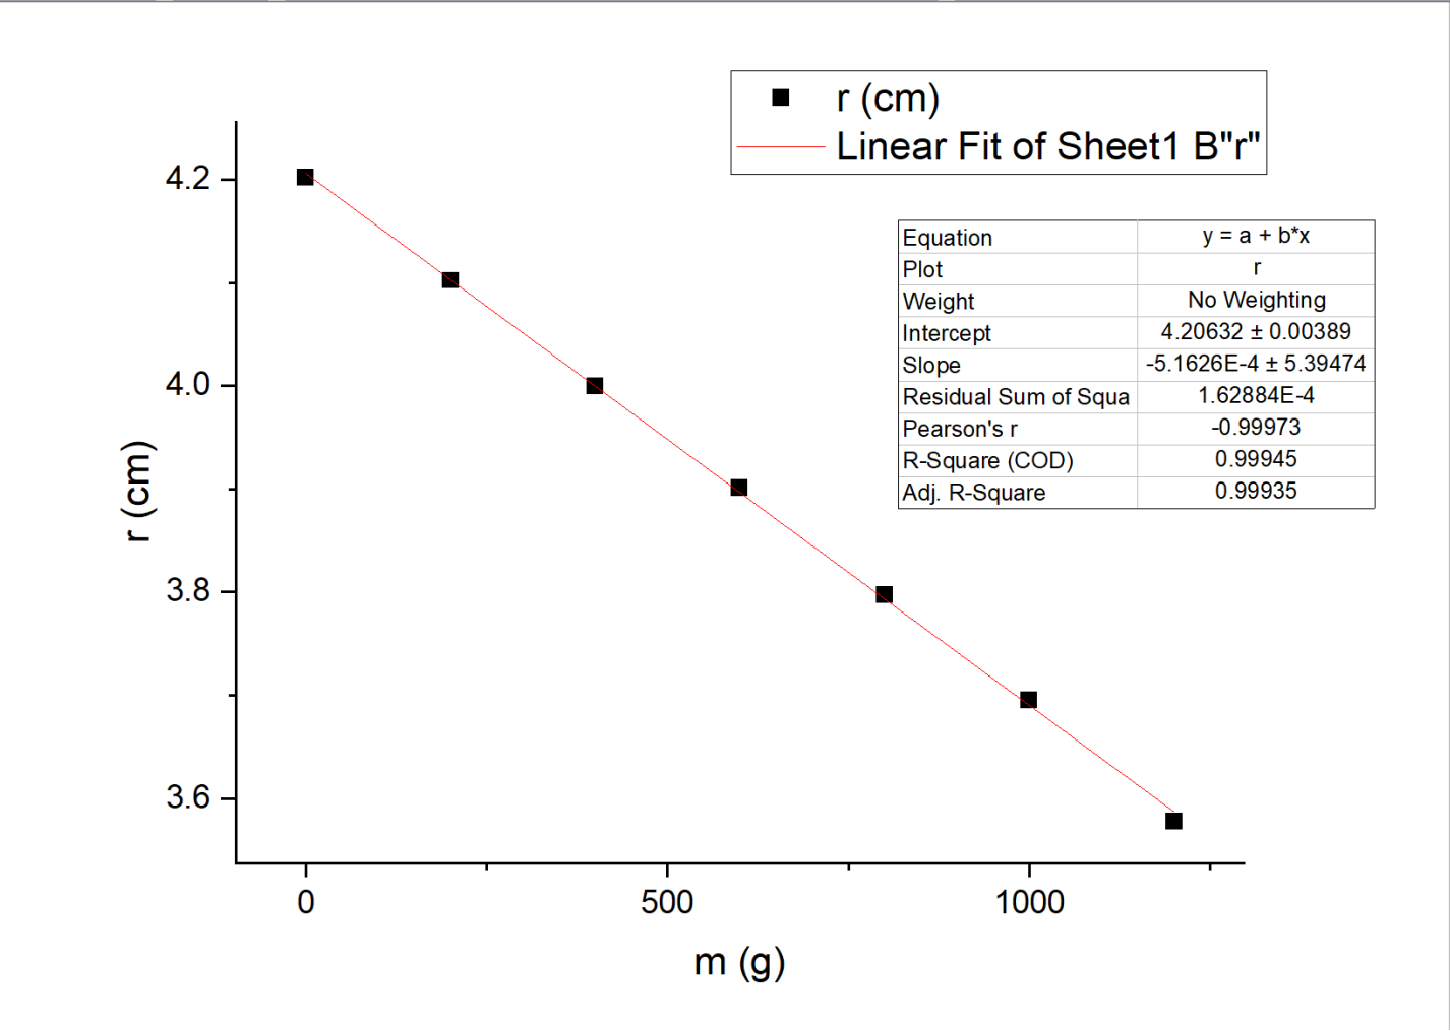
\includegraphics[width=.8\linewidth]{图片2.png}
	\caption{ 测得$ \bar{r} - m $关系图}
\end{figure}\noindent%
其中可以得到$$ a = -5.1626 * 10^{-4} $$
$$ b = 4.2063 $$
$$ r = -0.99973 $$

使用逐差法处理数据$$  \bar{\lambda} = \dfrac{(\bar{r_6} - \bar{r_3})+(\bar{r_5} - \bar{r_2})+(\bar{r_4} - \bar{r_1})+(\bar{r_3} - \bar{r_0})}{4} $$
$$ = \dfrac{0.3234 + 0.3045 + 0.3045 + 0.3014}{4} $$
$$ = 0.3035 cm $$
还有$$  \bar{\delta m} = \dfrac{(\bar{m_6} - \bar{m_3})+(\bar{m_5} - \bar{m_2})+(\bar{m_4} - \bar{m_1})+(\bar{m_3} - \bar{m_0})}{4} $$
$$ = \dfrac{599.25 + 599.70 + 600.10 + 600.40}{4} $$
$$ = 599.86 g $$
\subsubsection{计算杨氏模量}
根据公式计算得到
$$ \bar{\lambda} = 0.3035 cm $$
这里$g = 9.8012 N/kg$
$$ \bar{F} = \bar{\delta m} * g  = 5.8793 N  $$
其中有$$ \delta m = m_{i+3} - m_{i} $$
有杨氏模量的计算公式有
$$ E = \dfrac{F * L}{S * \delta L } $$
$$  = \dfrac{F * l^3 }{4* \lambda * a * h^3 } $$
$$ = 1.801 * 10 ^{11} N/m^2 $$



	


\section{分析与讨论}
\subsection{分析开始加第砝码时 r 的变化量大于正常的变化量}
     \begin{enumerate}
     	\item 在调试设备时,金属丝上下夹子未夹紧,在开始加第一、二个砝码时金属丝有一定的下滑。
     	\item 开始加第一、二个砝码时,金属丝有部分弯曲,第一、二个砝码不仅仅会拉长金属丝,还会把它拉直。
     	
     \end{enumerate}
    

	

	
\subsection{分析开始加第砝码时 r 的变化量小于正常的变化量}
    \begin{enumerate}
    	\item 开始加第一、二个砝码时,金属丝发生扭转,使金属丝拉长量减少。
    	\item 在调节设备时,没有调节好,使得开始加第一、二个砝码时,竖直方向有摩擦力的影响,使金属丝拉长量减少。
    	
    \end{enumerate}
	



	
\section{收获与感想}
\begin{enumerate}
	\item 在实验的过程中,要清楚逐差法的内核,笔者在计算CCD法测量的数据时,因为疏忽,计算了六个砝码的平均重量,但拉伸是在五个砝码的情况下发生的,因此导致E过大,更正错误之后,E的数值是正常的。注意逐差法在以后的实验中也有重要应用。
	\item 在CCD法测量的数据时,笔者在放第一个砝码时,金属丝没有发生伸长,发生了上面讨论的错误,以后应该注意。但在出现异常数据之后,将该数据舍去,笔者仍然得到了符合实际的E值。在以后的数据处理中,应该注意异常值的舍去。
\end{enumerate}



	\vfill\noindent\itshape\footnotesize
	\hfill Last edited: \today\ \copyright\ 赵启渊
\end{document}